\newpage
\begin{center}
    \textbf{\large 1. Preproduction}
\end{center}
\refstepcounter{chapter}
\addcontentsline{toc}{chapter}{1. РОЛЬ ДАЛЬНОДЕЙСТВИЯ ПРИТЯЖЕНИЯ В ПРОСТЫХ ЖИДКОСТЯХ}


\section{Обзор аналогичных решений}

\subsection{РБК}

\href{https://rbc.ru/}{РБК} --- один из крупнейший в России новостных ресурсах.

\begin{figure}[!ht]
    \centering
      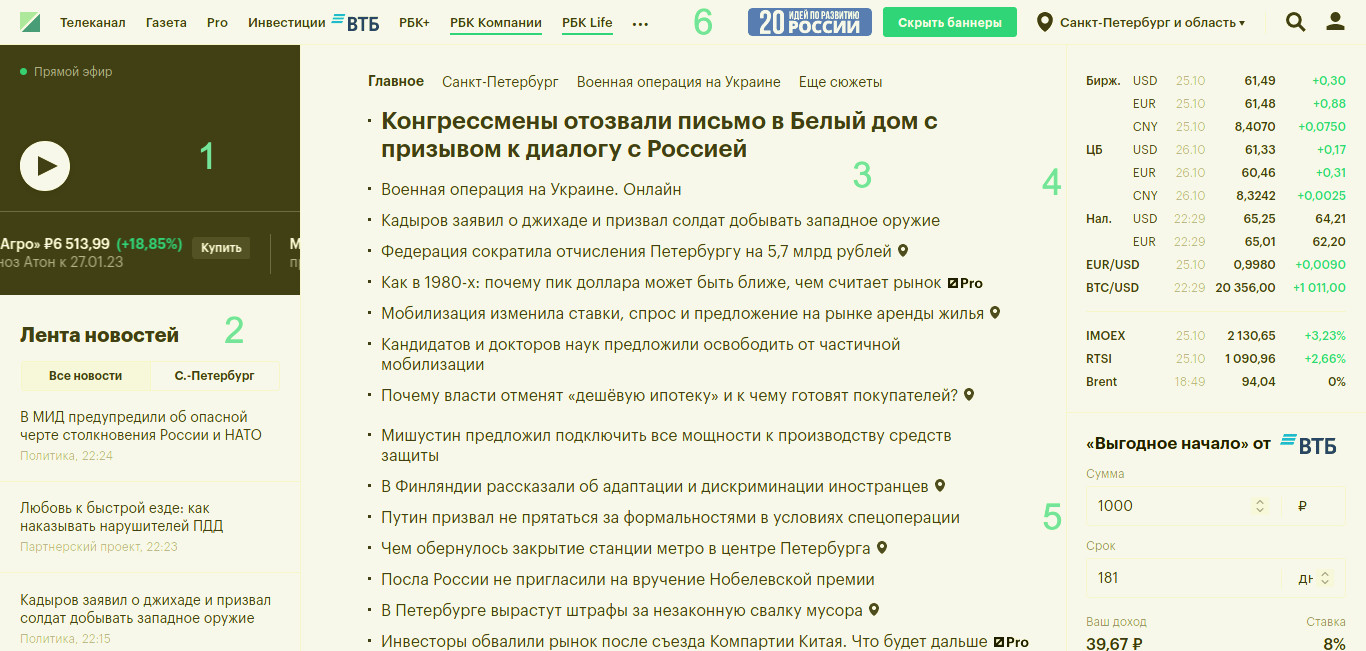
\includegraphics[width=1\linewidth]{./rbc/main-page.jpg}
      \caption{Главная страница ресурса \href{https://rbc.ru/}{rbc.ru}}
    \label{mainPage}
\end{figure}

На главная страницу портала: (1) трансляций телевизионного эфира; (2) столбец ленты новостей прокручивается вместе с основным содержанием и содержит рекламные объявления; (3) основной блок с еще одной секцией новостей, за которой при пролистывании следуют статьи портала; (4-5) самый крайний, третий столбец, вверху содержит котировки акций и рекламные объявления; (6) в "шапке" сайта выводится ссылки на другие разделы сайта и также на партнерские страницы.

На первый взгляд может показаться, что интерфейс сайта сложен для восприятия, однако, у меня при первом знакомстве с ним не возникло никаких сложностей. Благодаря грамотной работе с отступами, размерами элементов и сегментацией страницы дизайнерам удалось реализовать понятный пользовательский интерфейс. Кроме этого, они смогли разместить просто огромное количество информации на экране пользователя. И на мой взгляд, сайт перегружен данными, которые нужны далеко не всем группам пользователей - в ряд ли человеку, который пришел почитать новости, будет интересоваться стоимостью акций; а людям посещающим данный ресурс с целью мониторинга биржевых котировок, скорей всего, не заинтересуют прямая трансляция.

Открыв какую-нибудь статью для чтения, сегментации страницы останется не изменной - два столбца со сторонним содержим и сам материал (Рис.~\ref{articlePage}).

\begin{figure}[!ht]
    \centering
      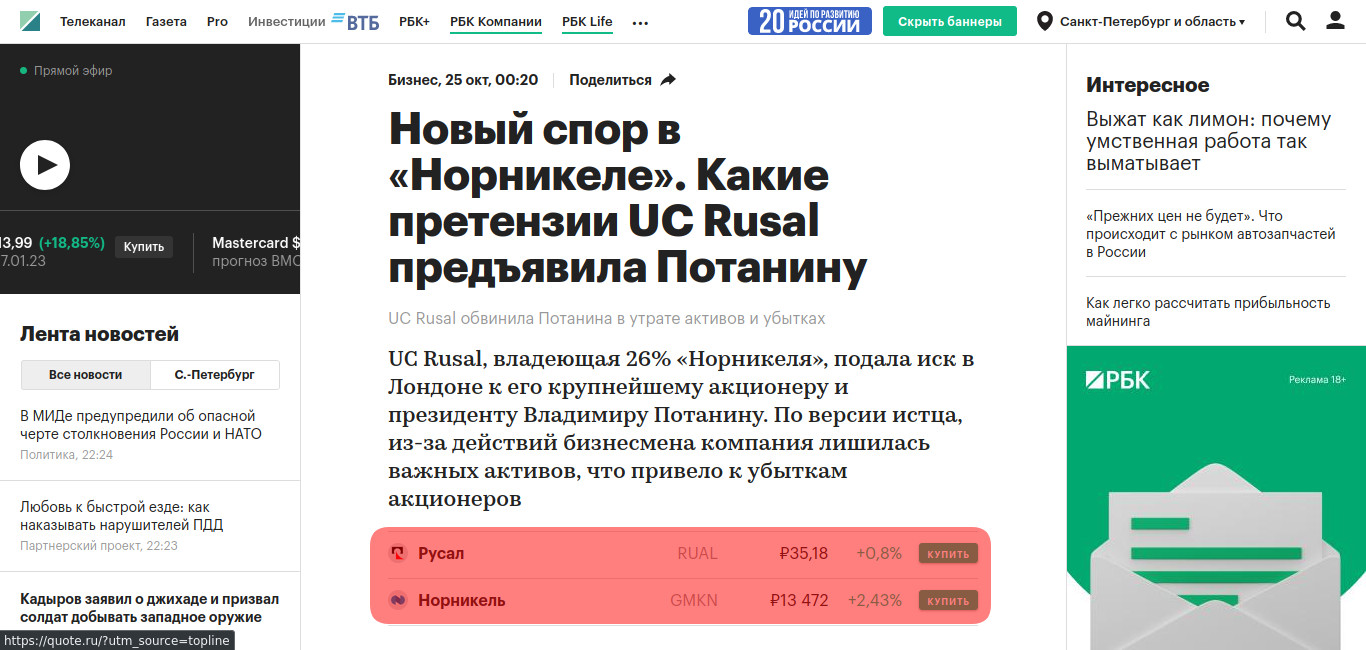
\includegraphics[width=1\linewidth]{./rbc/stocks-value.jpg}
      \caption{Страница статьи}
    \label{articlePage}
\end{figure}

Над заголовком, можно наблюдать \textbf{кнопку "поделиться"}, которая позволяет отправить ссылку на статью в одну из российских социальных сетей (Рис.~\ref{share}).

\begin{figure}[!ht]
  \centering
    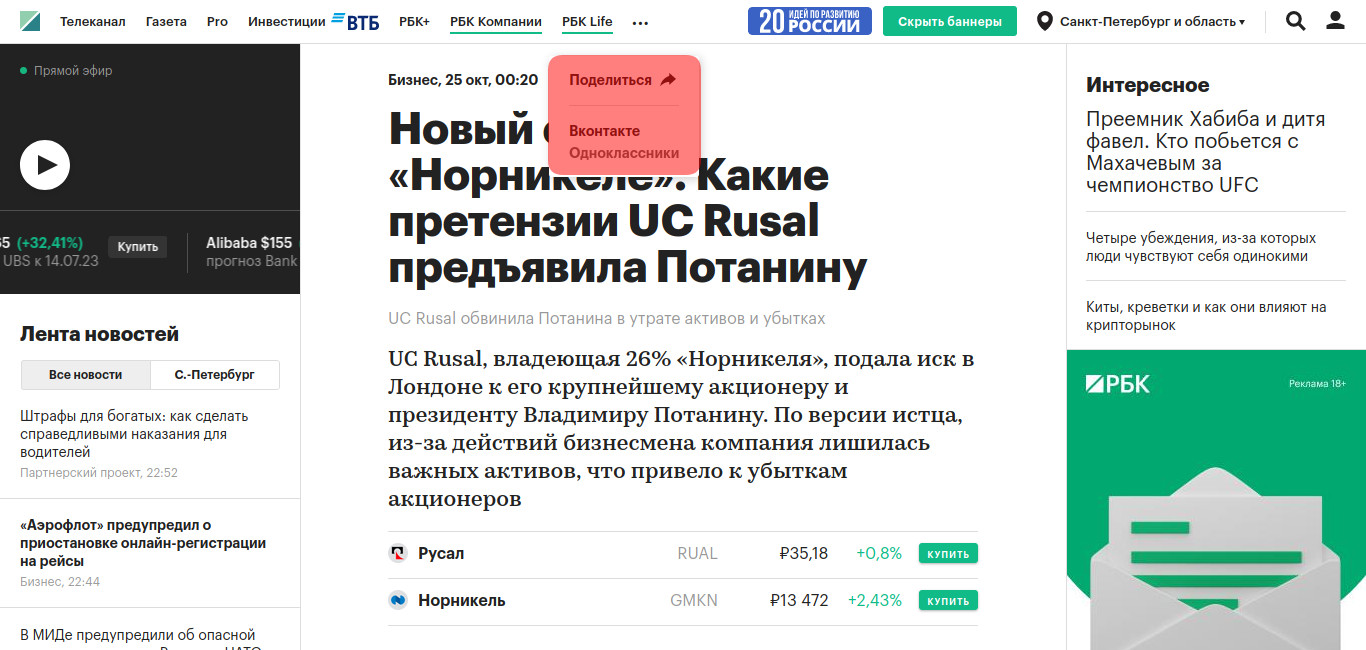
\includegraphics[width=1\linewidth]{./rbc/share.jpg}
    \caption{Раскрывающийся список всех ресурсов, в которые можно отправить ссылку}
  \label{share}
\end{figure}

При чтении основного содержания, нам будут постоянно предлагать ознакомиться с другими материалами (Рис.~\ref{suggestions}).

\begin{figure}[!ht]
  \centering
    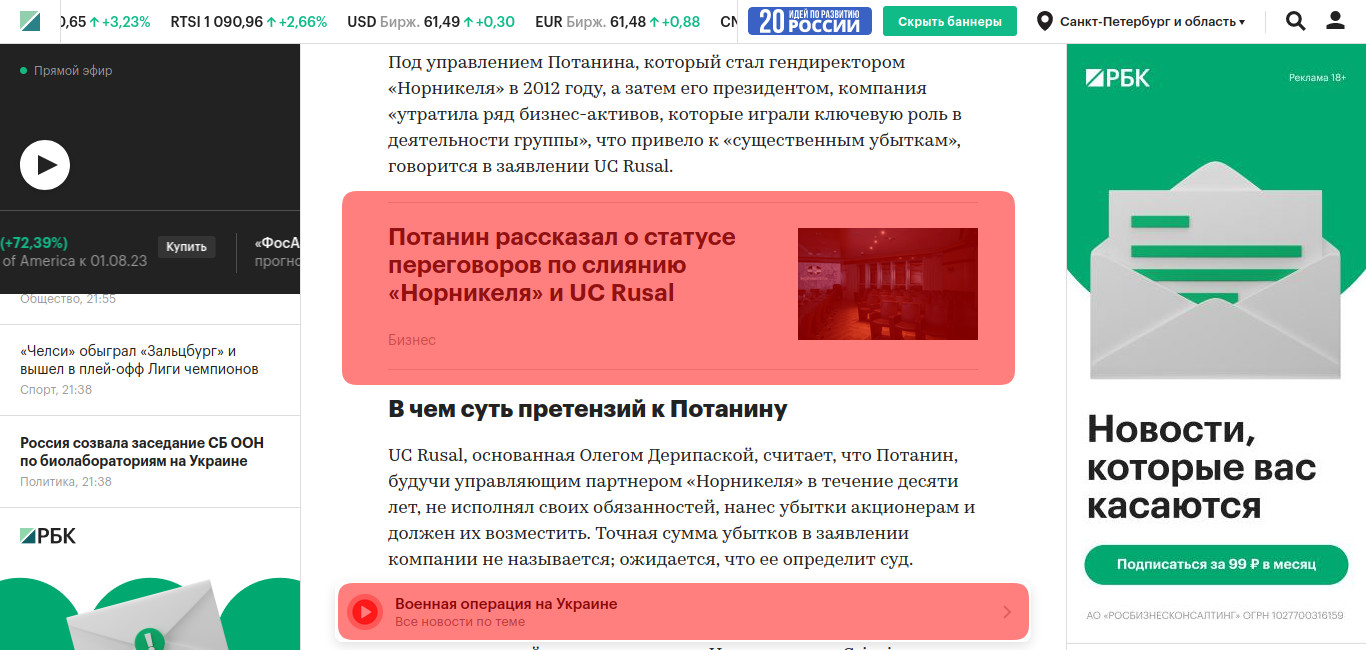
\includegraphics[width=1\linewidth]{./rbc/suggestion-to-read-articles.jpg}
    \caption{Предложения ознакомиться с другими статьями}
  \label{suggestions}
\end{figure}

Для меня, --- слишком много предложений, учитывая, что блок слева также выводит ссылки на другие статьи, хотя, очевидно, что при чтении на него пользователь обращает меньше внимания, и хотелось бы его убрать, оставив больше воздуха в самой статье.

В начале статьи находится блок со стоимостью ценных бумаг, который отображается в зависимости от содержания (\ref{stocks-value}).

\begin{figure}[!ht]
  \centering
    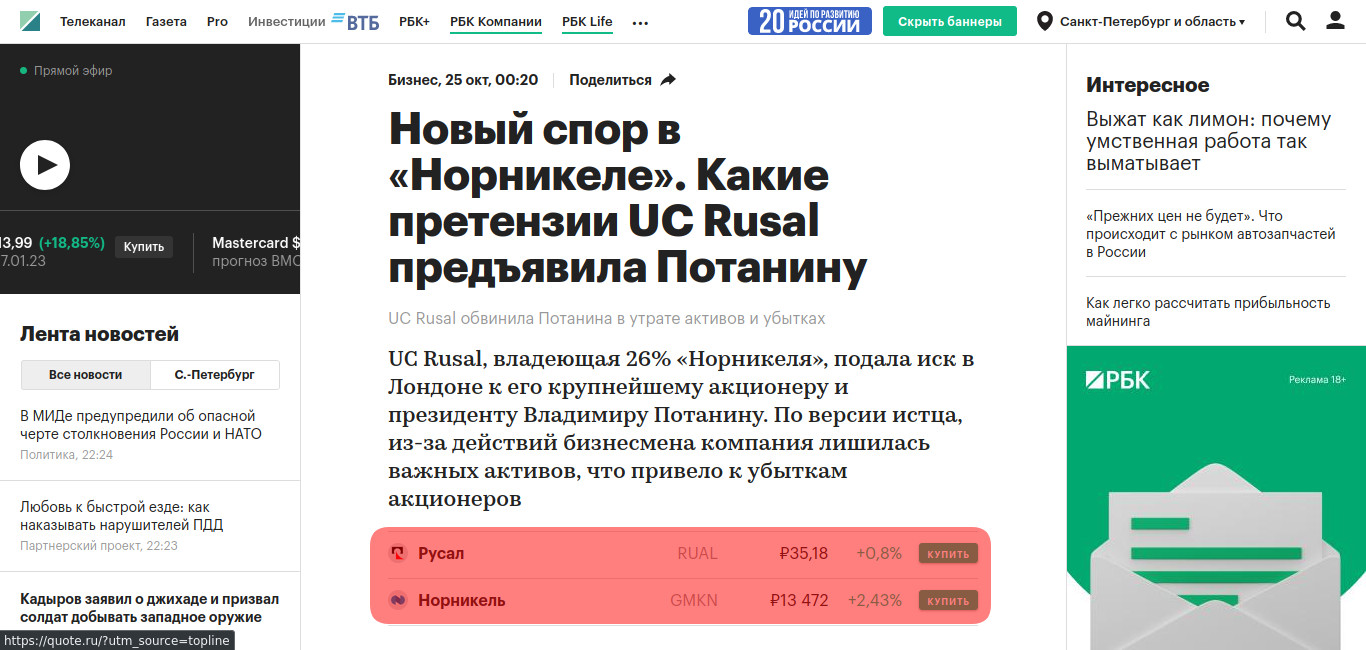
\includegraphics[width=1\linewidth]{./rbc/stocks-value.jpg}
    \caption{Блок стоимости ценных бумаг}
  \label{stocks-value}
\end{figure}

В правом блоке можно наблюдать предложение оформить платную подписку, которая позволяет получать рассылку на электронную почту (\ref{subscription}).

\begin{figure}[!ht]
  \centering
    \includegraphics[width=1\linewidth]{./rbc/subscribtion.jpg}
    \caption{Предложение оформить платную подписку}
  \label{subscription}
\end{figure}

\textbf{Если страница долистать до конца, то будут загружен новый контент}, что способствуют повышению удержания аудитории.


\subsection{Habr}

На \href{https://rbc.ru/}{habr.com} публикуются новости информационных технологий.

\begin{figure}[!ht]
  \centering
    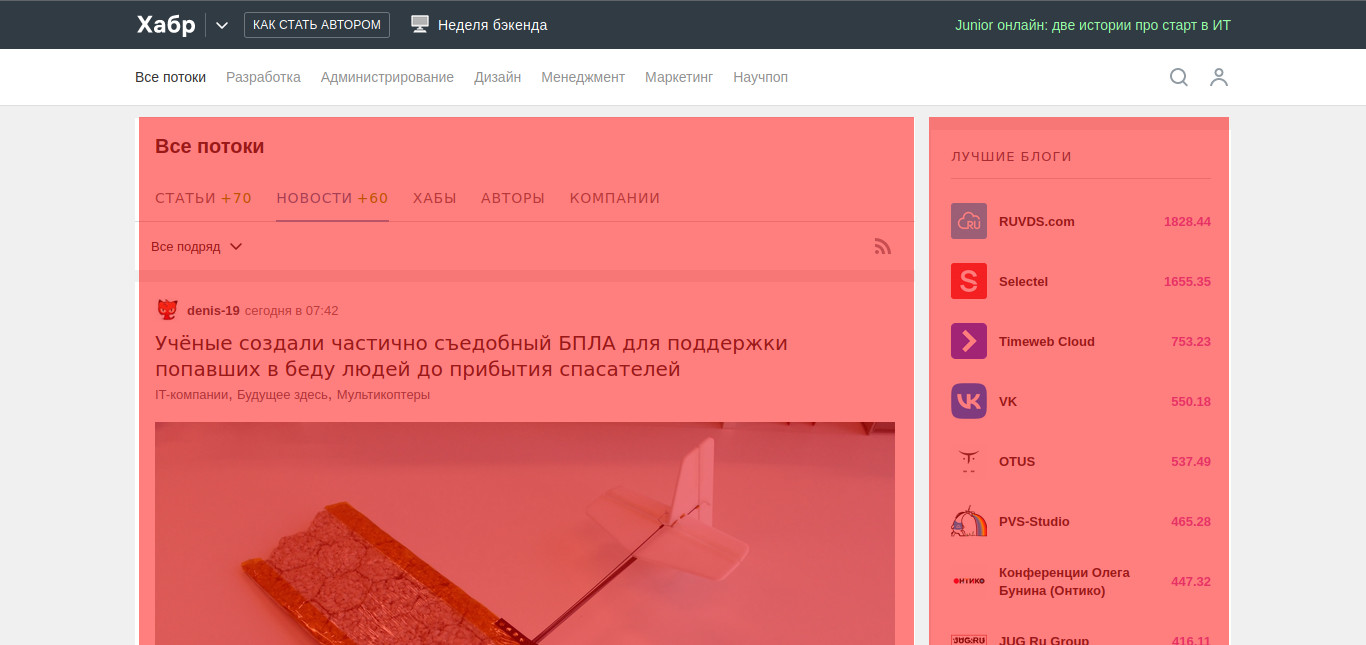
\includegraphics[width=1\linewidth]{./habr/two-column.jpg}
    \caption{Двуколонночная сетка сайта}
  \label{two-column}
\end{figure}

Открыв раздел с новостями, можно наблюдать разделение страницы на две части - основную, с новостями, и боковую со списками лучших блогов компаний, авторов, рекламными объявлениями и актуальными новостями (Рис.~\ref{two-column}).

Можно обратить внимание на то, что изображения к некоторым новостям слишком высокие и приходится прикладывать больше усилий, чтобы пролистать запись (Рис.~\ref{high-preview}).

\begin{figure}[!ht]
    \centering
      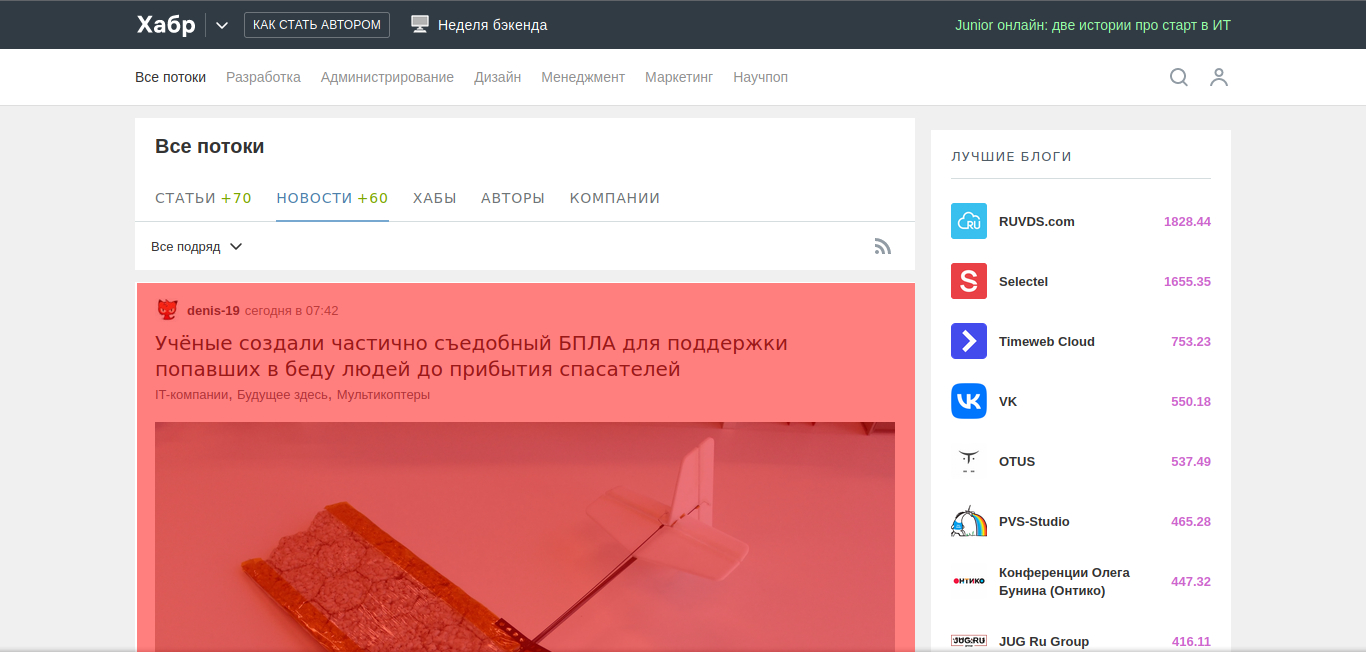
\includegraphics[width=1\linewidth]{./habr/high-preview.jpg}
      \caption{Пример записи с высоким изображением, не помещающейся на экране}
    \label{high-preview}
  \end{figure}

  Карточка публикация состоит из ссылки на профиль автора (1), даты и времени публикации (2), заголовка (3) и категорий (4), к которым относится публикация, изображения (5), краткого содержания (6), кнопки "Читать далее" (7) для перехода к основному содержанию (на мой взгляд она тут лишняя), а также небольшая статистическая сводка - рейтинг, количество комментариев, просмотров и людей, добавивших публикацию в закладки (Рис.~\ref{post-structure}). 

  \begin{figure}[!ht]
    \centering
      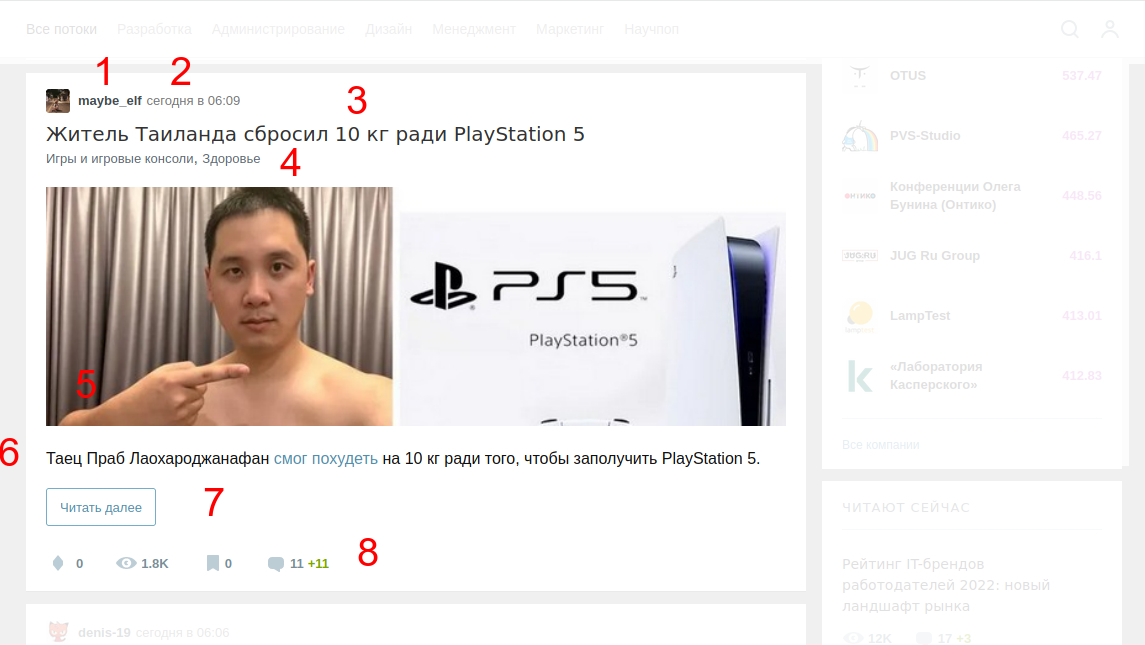
\includegraphics[width=1\linewidth]{./habr/post-structure.jpg}
      \caption{Структура записи}
    \label{post-structure}
  \end{figure}

  По мере просмотра новостной ленты, нам будут встречаться дополнительный материал напрямую не относящийся к новостям, например, "Истории" --- ещё один канал доставки информации от разработчиков ресурса до читателей с привлекательными картинками и ссылками на основную запись. Так же могут встречаться рекламные блоки, ссылки на заказы на freelance.habr.com и различная статистическая информация.

  \begin{figure}[!ht]
    \centering
      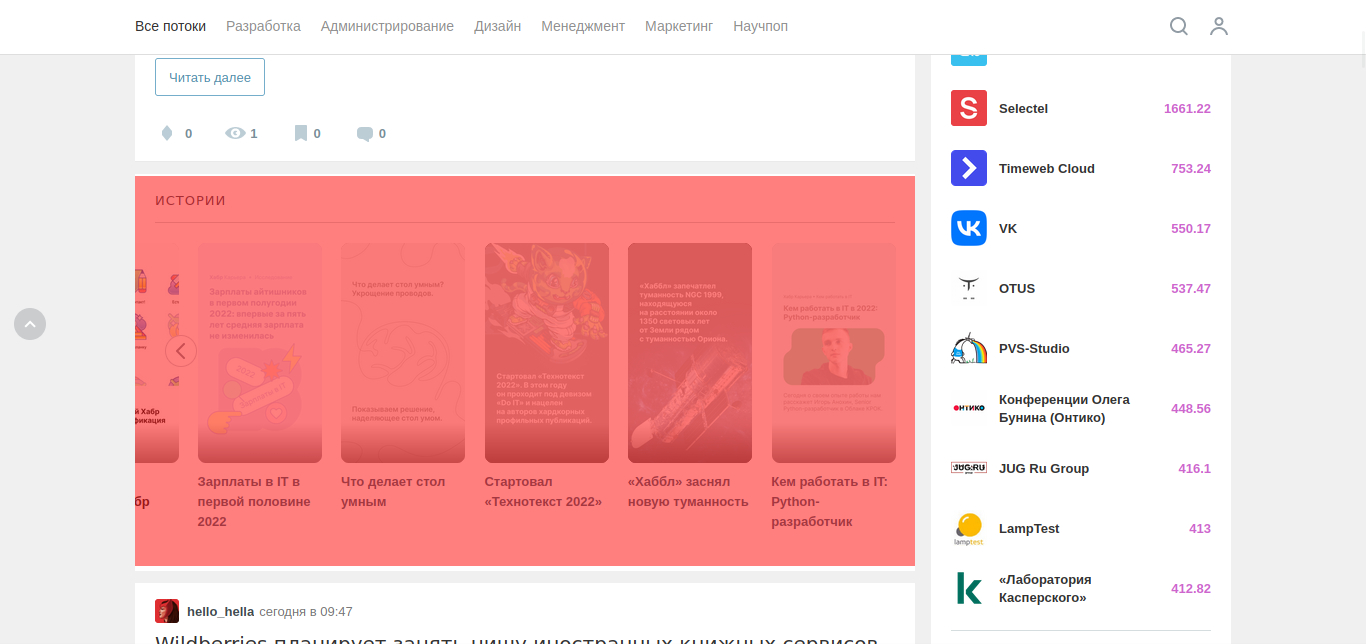
\includegraphics[width=1\linewidth]{./habr/stories.jpg}
      \caption{Блок "Историй"}
    \label{stories}
  \end{figure}

  Новостная лента не бесконечная --- в конце находится пагинация.

  \begin{figure}[!ht]
    \centering
      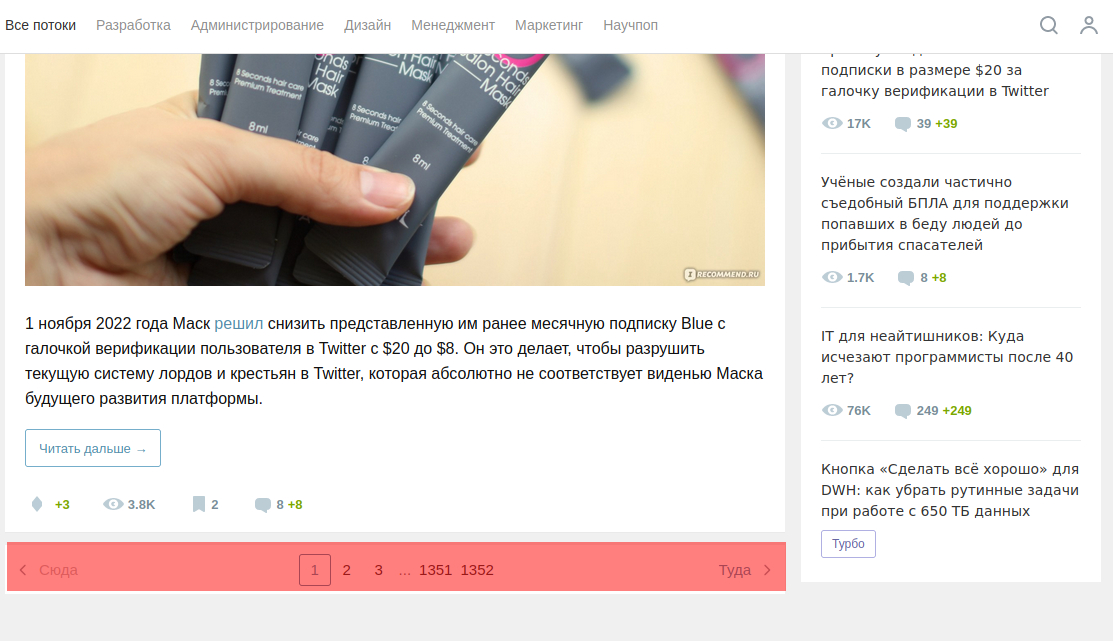
\includegraphics[width=1\linewidth]{./habr/pagination.jpg}
      \caption{Пагинация}
    \label{pagination}
  \end{figure}

  На самой странице новости всё стандартно - основное содержимое, изображения, ссылки и так далее. Однако в конце можно увидеть список тегов, которые, скорей всего, используется при ранжировании новости в поисковых системах и на самом сайте, а так же \textbf{едва заметную кнопку "поделиться"}.

  \begin{figure}[!ht]
    \centering
      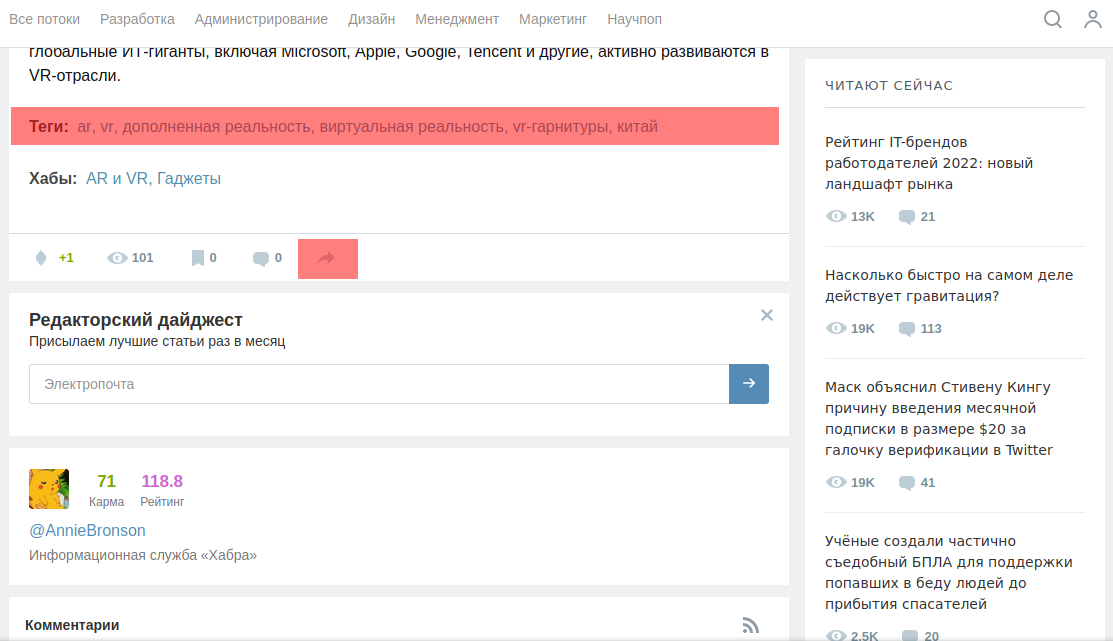
\includegraphics[width=1\linewidth]{./habr/tags.jpg}
      \caption{Список тегов и кнопка поделиться}
    \label{tags}
  \end{figure}

  Здесь же расположился блок оформлениея бесплатной e-mail рассылки.

  \begin{figure}[!ht]
    \centering
      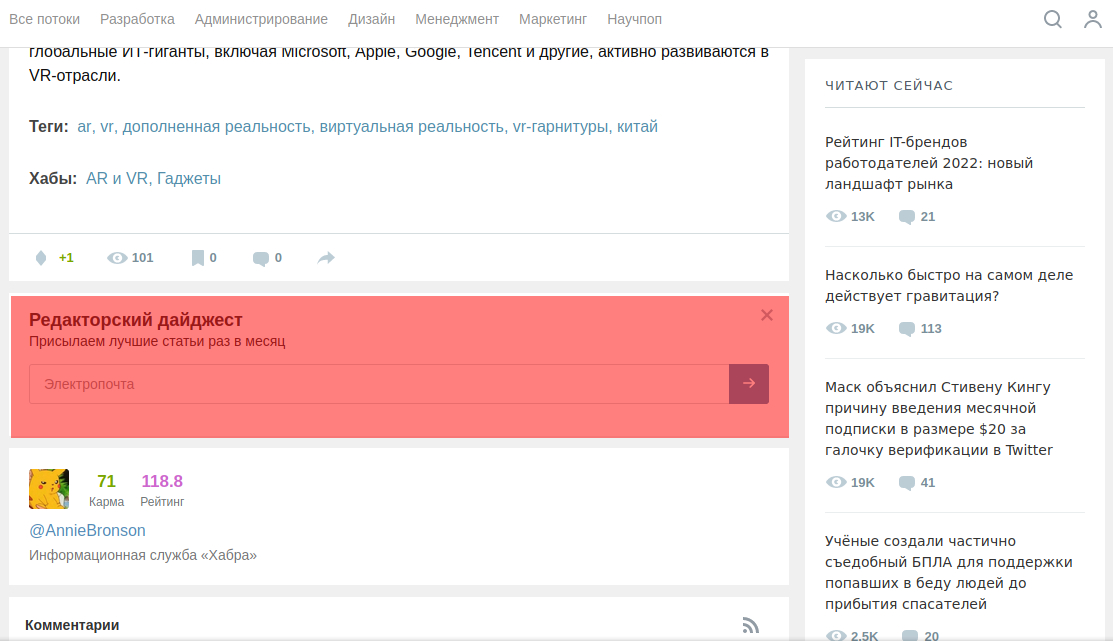
\includegraphics[width=1\linewidth]{./habr/subscription.jpg}
      \caption{Секция e-mail рассылки}
    \label{habr-subscription}
  \end{figure}

  \subsection{DTF}

  \href{https://dtf.ru/}{dtf.ru} --- новостной ресурс об видео-играх и их разработке, на котором публикуются статьи редакции и пользователей. Функционал сайта и его внешний вид схожи с предыдущими ресурсами, однако хочу отметить локаничность карточки записи.

  \begin{figure}[!ht]
    \centering
      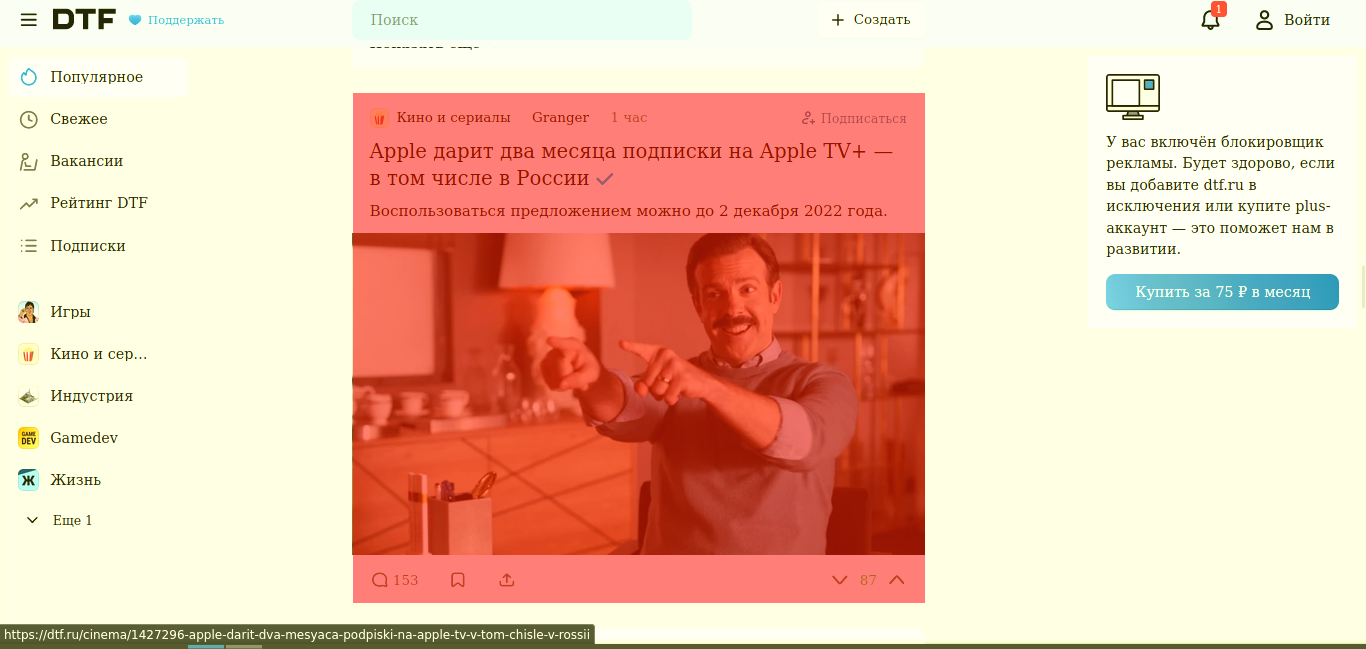
\includegraphics[width=1\linewidth]{./dtf/minimal-post-card.png}
      \caption{Минималистичная краточка записи}
    \label{minimal-post-card}
  \end{figure}

  Так же это один из немного новостных ресурсов, который позволяет зарегестрированным пользователям подписать на публикации интересующего их автора.

  \begin{figure}[!ht]
    \centering
      \includegraphics[width=1\linewidth]{./dtf/subscribtion.jpg}
      \caption{Минималистичная краточка записи}
    \label{dtf-subscribtion}
  \end{figure}

  Также стоит отметить, что человек, вошедший в свой аккаунт на dft, может оставлять \textbf{комментарии} под публикациями. Такая же возможность есть и на упоминаемом выше habr.com.

  \begin{figure}[!ht]
    \centering
      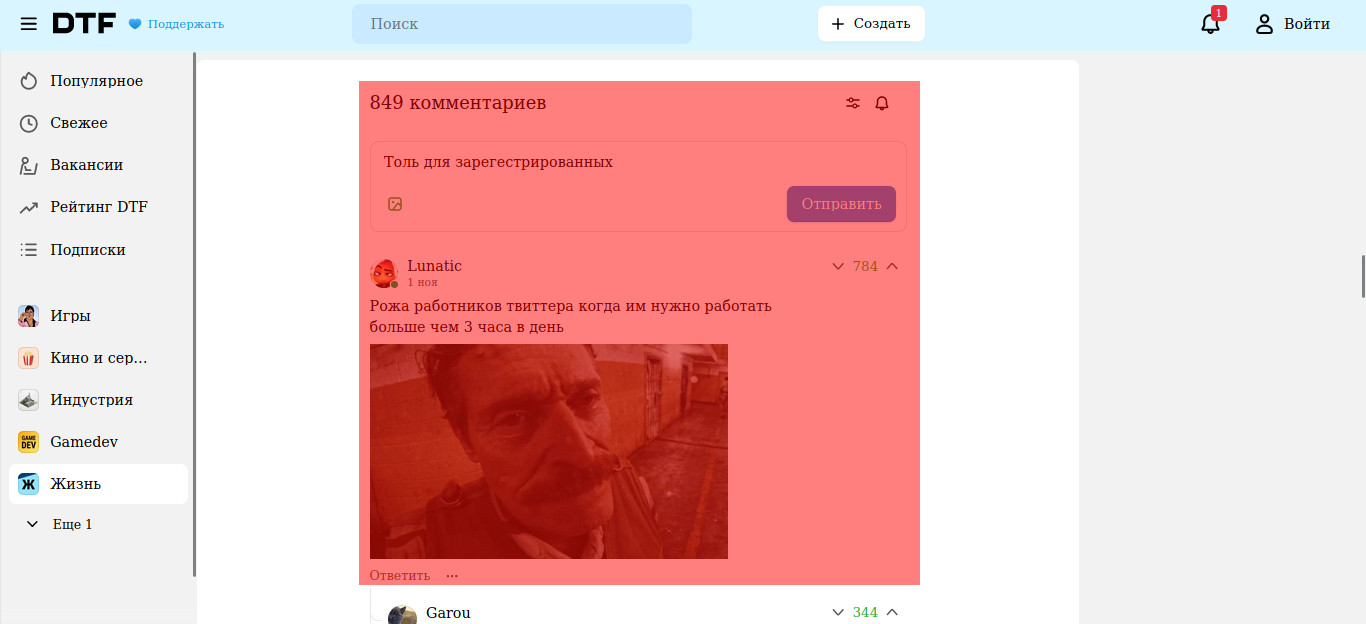
\includegraphics[width=1\linewidth]{./dtf/comments.jpg}
      \caption{Минималистичная краточка записи}
    \label{dtf-comments}
  \end{figure}

  \subsection{Антипримеры}

  Остальные новостные ресурсы и агригаторы такие как Google News и Яндекс.Новости плюс минус одинаково выглядят и имеют похожий функционал - поделиться в социальных сетях, статистика просмотров и активности, теги, темы и т.д. Однако для себя я нашел несколько антипримеров.

  \begin{figure}[!ht]
    \centering
      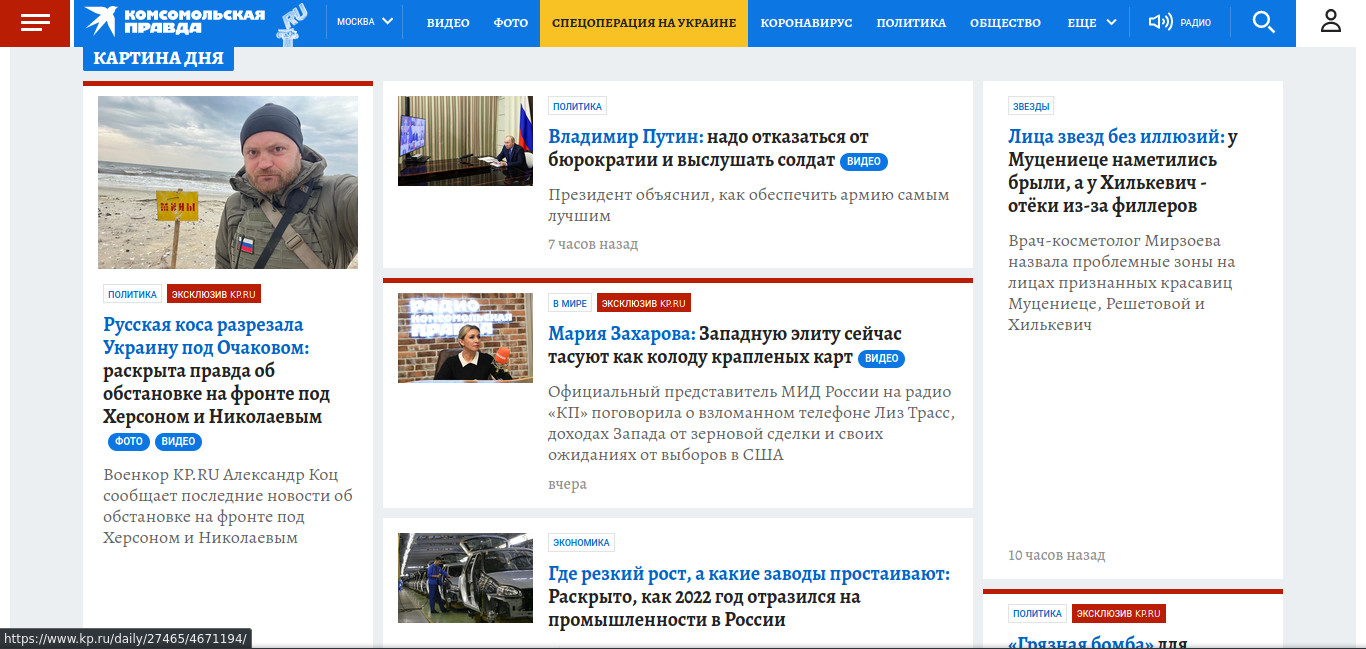
\includegraphics[width=1\linewidth]{./antiexamples/kp.jpg}
      \caption{Страница "Комсомальской правды"}
    \label{kp}
  \end{figure}
  
  По моему мнению, на сайте \href{https://www.kp.ru/}{kp.ru} акценты выставлены не совсем корректно. Огромную часть внимания привлекает "шапка" ярко-синего цвета. Кроме этого, для чего-то очень явно акцентируют новостные метки такие как "видео" и "фото". Сложно сказать зачем это было сделано, учитывая что сейчас пользователя сложно удивить только лишь наличием первого и второго. Также я не вижу необходимости выделять часть заголовка цветом.

  \begin{figure}[!ht]
    \centering
      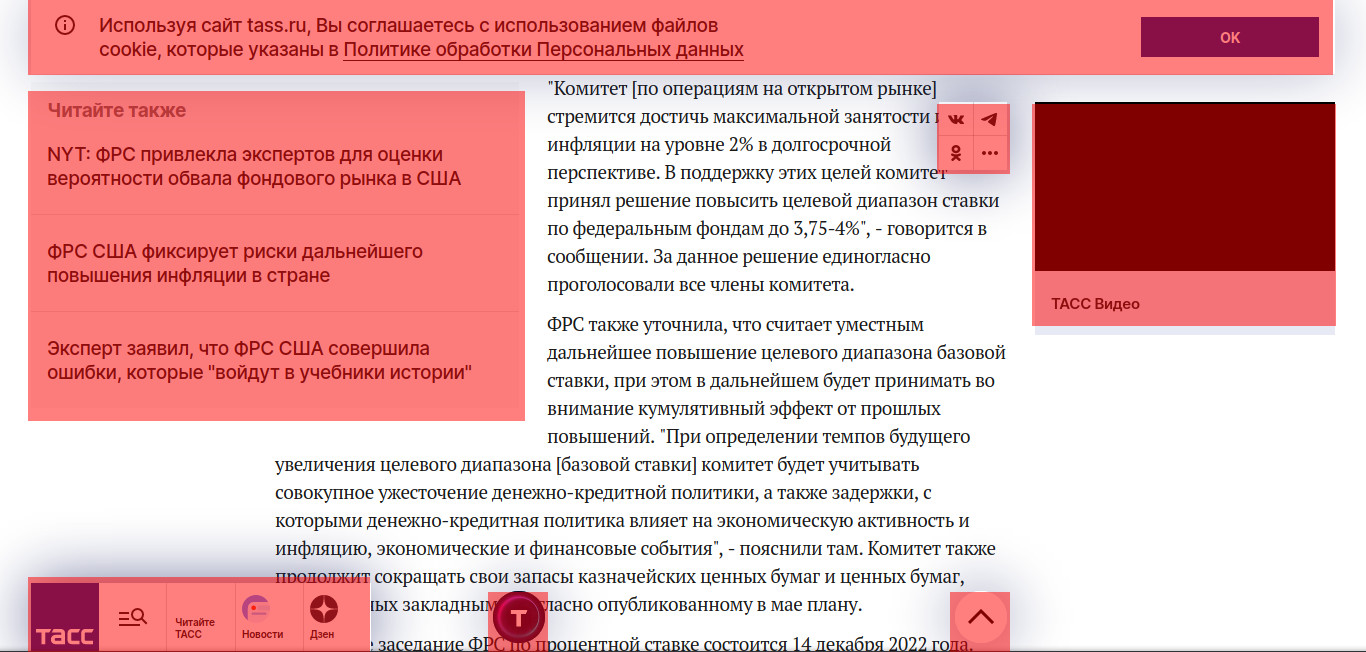
\includegraphics[width=1\linewidth]{./antiexamples/tass.jpg}
      \caption{Страница новости на ТАСС}
    \label{tass}
  \end{figure}

  Страница с содержанием публикации на \href{https://tass.ru/}{ТАСС} дала мне явно понять, что пользователю ничего не должно мешать читать.

  \section{Ключевые особенности проекта}

  \subsection{Проблема и ключевая особенность приложения}

  На всех рассмотренных ранее новостных ресурсах пользователь мог подписаться на e-mail рассылку. В большинстве случаев это бесплатно, так как это позволяет установить "диалог" с читателем, что в конечном счете так или иначе конвертируется в прибыль, однако встречались исключения, например, РБК, где за подписку нужно платить. Всё бы ничего, но на мой взгляд, электронная почта не лучшее место для потребление контента, потому что практически всегда e-mail используется для регистрации на тех или иных сайтах, которые зачастую "спамят"  пользователь не интересующими его письмами. И велика вероятность, что материал, доставляющийся человеку таким способом, будем им незамечен в том хаусе не прочитанных сообщений.

  Альтернативный вариант предоставлять пользователю обновления - это широко распространенный механизм подписка, который был реализован на \href{http://dtf.ru}{DTF}, а так же во популярных социальных сетях. Но такое решение не подходит мало популярным или только-что запущенным интернет ресурсам из-за необходимости регистрации аккаунта - сложно заставить человека создать его, если он не пользуется ресурсом достаточно часто.

  Решением описанных выше проблем я вижу в механизме доставке контента на массовые платформы, --- социальные сети и месенджеры. Из рассмотренных ранее, достаточно популярных, новостных ресурсов ни один из них не предлагал пользователю оформить рассылку в его любимую социальную сеть или мессенджер, хотя практически каждый новостной ресурс имеет свое сообщество на тех или иных платформах. Так же стоит отметить, что за всё проведенное мной время в глобальной сети я ни разу не встречал сайт, позволяющий сделать это.

  Механизм доставке контента будет разрабатываться в контексте новостного портала.

  \subsection{Функционал новостного портала}

  Большинство пользователей Интернета не читают новости дальше заголовка. Поэтому основная идея данного проекта - это разработать новостной портал, на котором новости \textbf{состоят только из одного заголовка} и \textbf{небольшого, необязательного, комментария автора}.

  В ходе обзора аналогов я не встретил ни одного ресурса, на котором бы список источников был бы выделен в отдельные блок. Учитывая, что новостные порталы по большей части являются ретрансляторами информации, \textbf{считаю необходимым более явно выделять ссылки на исходные материалы}, для того чтобы пользователь всегда мог ознакомиться с оригиналом. В контексте разрабатываемого проекта вынести список источников в отдельный блок - хорошая идея, так как у автора появляется очень простой способ раскрыть тему, просто прикрепив ссылку на источник. Так же это дает позволяет читателям ознакомиться с тем или иным материалом более подробно.

  Еще одна ключевая особенность разрабатываемого новостного ресурса, заключается в том, что \textbf{}{любой} пользователь - зарегистрированный и нет - \textbf{может просматривать и оставлять комментарии к записям}. Это должно повысить увлеченность читателей.

  \begin{figure}[!ht]
    \centering
      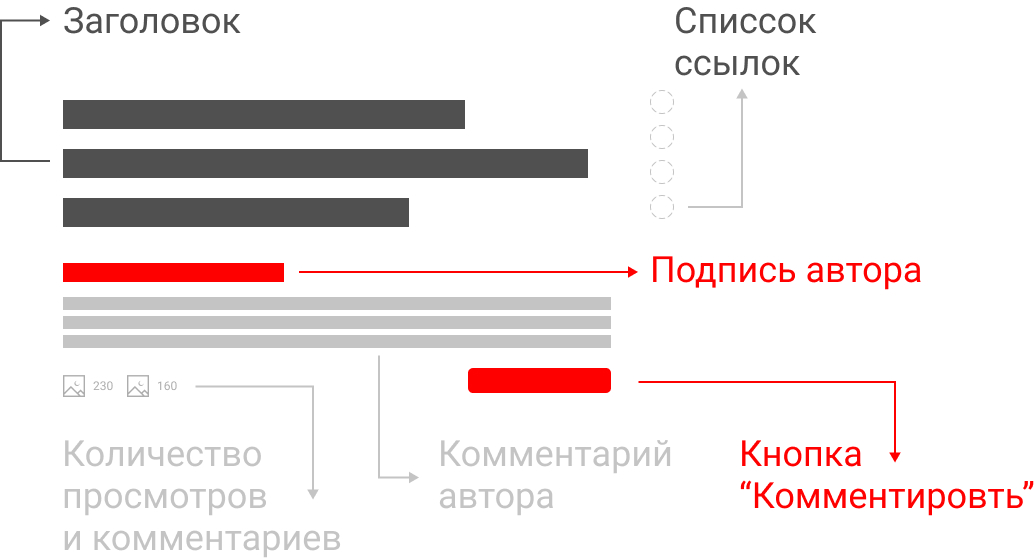
\includegraphics[width=1\linewidth]{./desing-prototypes/news-prototype.jpg}
      \caption{Дизайн-протатип новостной записи}
    \label{news-prototype}
  \end{figure}

  В рассмотренных ранее аналогах не каждый пользователь мог написать и опубликовать статью на ресурсе. Для этого ему нужно было пройти модерацыию. Считаю реализовать похожий механизм. Чтобы получить доступ к публикации записей, пользователь сначала должно \textbf{отправить заявку на авторство}. В случаи ее одобрение, он может \textbf{создать аккаунт}, после чего \textbf{писать и публиковать новости}.

  Неотъемлемы функционала любого сайта является возможность \textbf{писать и публиковать новости}{поделиться записью} со своими друзьями. Текущий проект не станет исключением. Это должно положительно сказать на росте популярности ресурса.

  \textbf{В случаи наличия достаточных временных ресурсов}, планирую реализовать \textbf{PWD-приложения}. Это должно повысить посещаемость портала. А так же \textbf{механизм категорий}, что пользователям читать новости на интересующие их темы.